\documentclass[11pt,a4paper,twoside,notitlepage]{article}
%comment out the line above and decomment the one below; the format will change
%\documentclass[conference,a4paper]{IEEEtran}  

%
% Here, you specify the packages you need
%

%You need these 2 packages to write algorithms
\usepackage{algorithmic}
\usepackage{algorithm}
%You need this package to handle figures
\usepackage{graphicx}
%You need this package to write Romanian diacritics properly
\usepackage{combelow}
\usepackage{hyperref}

\usepackage[utf8x]{inputenc} %alternative solution for Romanian diacritics
%This is how you define you own commands/macros
%this is a macro for writing "n choose k" the Romanian style
\newcommand{\mycomb}[2]{{C}_{#1}^{#2}} 
%this is a macro for writing "n choose k" the English style
%\newcommand{\mycomb}[2]{\left( \begin{array}{l}{#2}\\{#1}\\ \end{array} \right)} %this 


%
% The document content starts here
%
\setcounter{tocdepth}{2}
\renewcommand{\contentsname}{Cuprins}
%\setlength{\parindent}{4em}

\begin{document}
% paper title 
\title{Bontida part 3}

% author names and affiliations
\author{
Student: Gabor George C\u{a}t\u{a}lin\\ %double backslash means linebreak
Grupa: 30239\\
}

%generate paper title
\maketitle 

\newpage

\tableofcontents

%\section*{Cuprins}


\newpage

\section{Analiza cerințelor}

\subsection{Specificare cerinte}
Se cere realizarea părții de "Back-end" pentru o aplicație mobile pentru a oferi informații participanților la fectivalul Electric Castle. \par
	Aplicația trebuie să fie construită pe baza arhitecturii Service Oriented Architecture (SOA), av\^u{a}nd un serviciu Web principal care expune un API aplicației mobile și două servicii ce vor fi folosite de cel principal. Primul va returna informații legate de artiști iar al doilea informații legate de vreme.

\subsection{Cerinte functionale}
Aplicația trebuie să pună la dispoziție utilizatorilor următoarele funcționalități:
\begin{itemize}
	\item GET http://localhost/api/artists
		\begin{itemize}
			\item Returneaza o lista cu toate trupele
		\end{itemize}
	\item GET http://localhost/api/artists?stage=\textless stage\_name\textgreater
		\begin{itemize}
			\item Returneaza o lista cu toate trupele care vor canta la scena \textless stage\_name\textgreater
		\end{itemize}
	\item GET http://localhost/api/artists?day=\textless day\_nr\textgreater\&hour=\textless hour(5-10)\textgreater
		\begin{itemize}
			\item Returneaza o lista cu toate trupele care vor canta la data si ora respectiva
		\end{itemize}
	\item GET http://localhost/api/artists?artistname=\textless artist\_name\textgreater
		\begin{itemize}
			\item Returneaza scena, ziua, ora + vremea de la ora respectiva

		\end{itemize}
\end{itemize}

\subsection{Cerinte non-functionale}
Urmatoarele cerinte trebuie respectate:
\begin{itemize}
	\item 	utilizarea unui framework ce implementează patternul MVC (Spring Boot);
	\item	serviciul principal trebuie implementat prin agregarea a două servicii secundare;
	\item 	servicile secundare vor fi create utiliz\^{a}nd https://sheetsu.com/;
	\item 	utilizarea pattern-ului Chain of Responsibility;
	\item	utilizarea arhitecturii SOA;
	\item 	implementarea funcționalității de cache cu timp de expirare a datelor asupra informaților returnate de servicile secundare;
	\item 	utilizare https://sheetsu.com pentru crearea API de returnare date despre artiști și vreme.
\end{itemize}

\section{Use Case Model}

Use case: Vizualizarea artiștilor ce au spectacol pe o scenă; \\
Level: User-goal; \\
Actor princital: Dispozitivul mobil; \\
Scenariu de succes: În browser este introdusă adresa \\ http://localhost:8080/api/artists?stage=\textless User\_Input \textgreater. Aplicația va căuta în cache informațile și dacă nu sunt prezente sau a trecut suficient timp va face o cerere la serviciul ce returneză informații despre artiși. Apoi se face o filtrare a artiștilor dupa scenă și se returnează numelor celor ce corespund. \\
Extensii: Operatia poate eșua dacă:
\begin{itemize}
	\item intervine o problemă cu serviciul de informații pentru artiști.
\end{itemize}

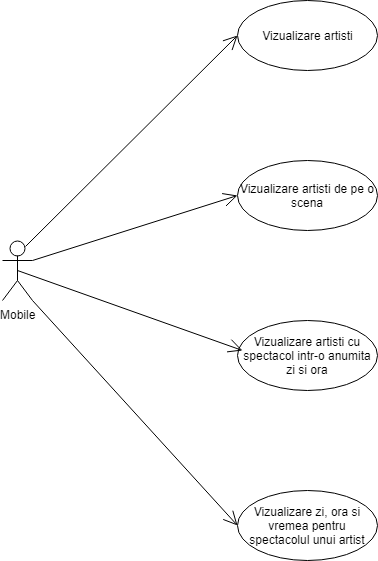
\includegraphics[height=.5\textheight]{useCases}


\section{Design-ul arhitectural al sistemului}

\subsection{Descrierea modelului arhitectural}
Este utilizat pattern-ul arhitectural MVC.\\
Aplicatia este compusa din două nivele: 
\begin{itemize}
	\item Controller - leaga Modelul de View și procesează toate cererile;
	\item Model - oferă acces structurat la date. 
																	\begin{itemize}
																		\item Entities - structurile de date;
															
		\item Services - combină Entities și Repositories pentru a returna date structurate.
																	\end{itemize}
\end{itemize}

Deasemenea este utilizat Service Oriented Architecture, aplicația utiliz\^{a}nd două servicii:
\begin{itemize}
	\item EC\_artists - access informații artiști;
	\item EC\_weather - access infromații vreme.
\end{itemize}


\subsection{Diagrame}

Urmatoarea diagrama prezinta structura pachetelor din sistem : \\
\\
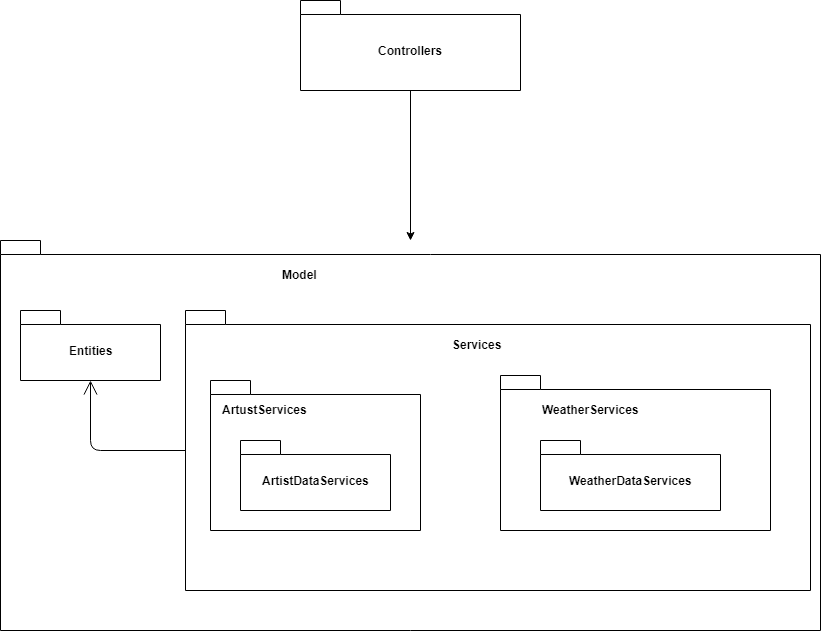
\includegraphics[height=.4\textheight, width=.8\textwidth]{packages} \\
\\
Diagrama de componente: \\
\\
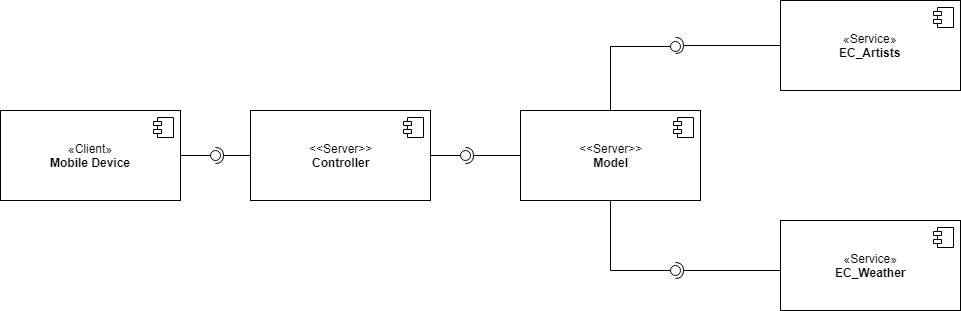
\includegraphics[width=.6\textheight]{components} \\
\\
Diagrama de deployment: \\
\\
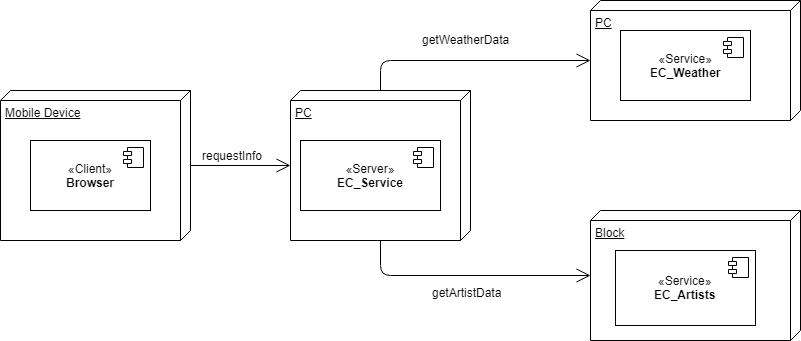
\includegraphics[width=.6\textheight]{deployment} \\


\section{Diagrame de secventa UML}
Consideram scenariul în care se face o cerere de returnare a artiștilor ce au spectacol pe o anumită scenă: \\ \\
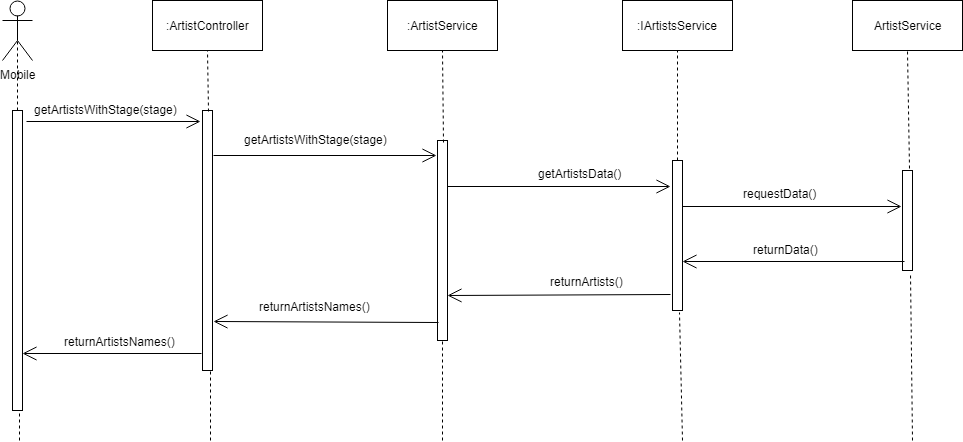
\includegraphics[width=.6\textheight]{secventa}


\section{Design-ul claselor}

\subsection{Descriere design pattern-uri utilizate}

Au fost utilizate urmatoarele:
\begin{itemize}
	\item Chain of responsability - Clasa EcArtistsCachedService returnează în mod normal datele despre artiști, dau uneori cere clasei EcArtistsWebService datele pentru a le reîmprospăta. Comunicarea se face utiliz\^{a}nd interfața IArtistsService.
	\item Composite - WeatherDetails are ca atribut o instanță a clasei ArtistDetails;
\end{itemize}

\subsection{Diagrama de clase}
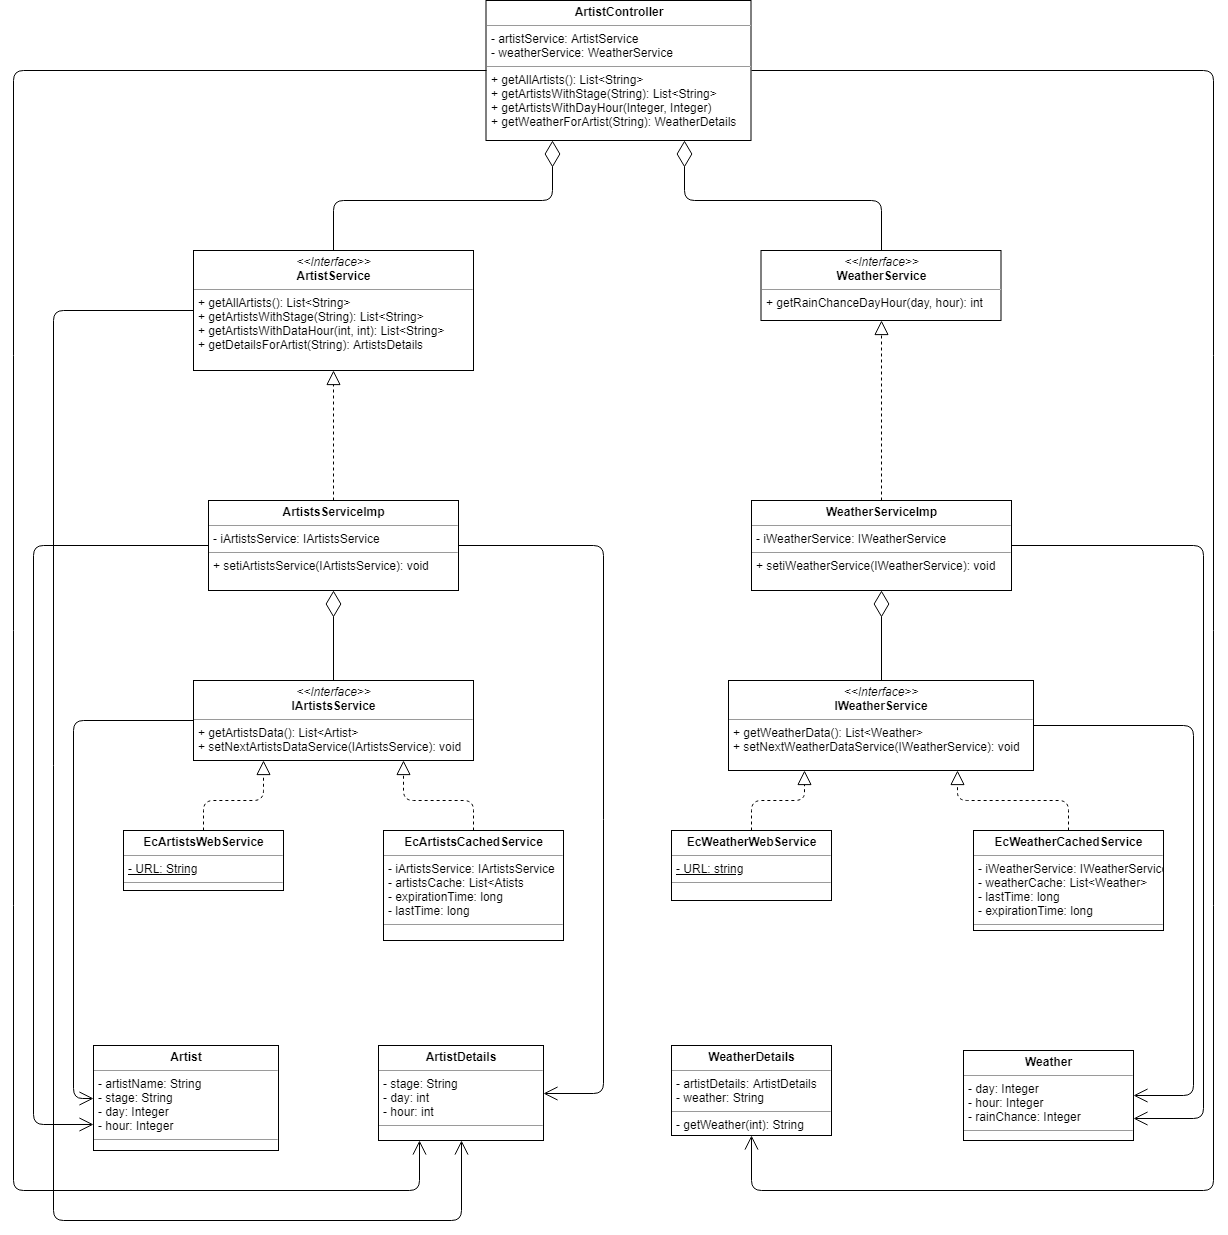
\includegraphics[height=.7\textheight, width=1.3\textwidth]{class}
\newpage

\section{Model de date}

Datele au fost stocate utiliz\^{a}nd Google Spreadsheet. Tabelele av\^and următoarea formă: \\ \\
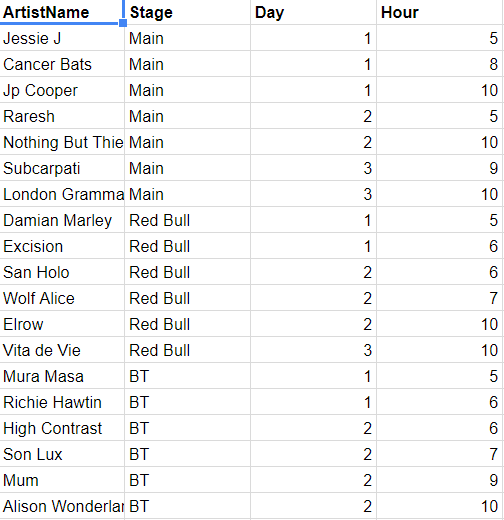
\includegraphics[height=.4\textheight, width=.6\textwidth]{artisti} \\ \\
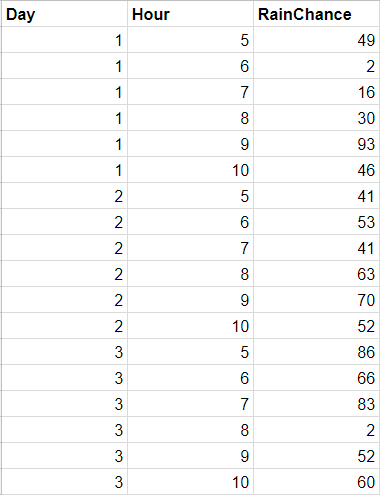
\includegraphics[height=.35\textheight, width=.5\textwidth]{vreme} \\



\section{Testarea sistemului}

S-a folosit o strategie de testare incrementală, funcționalitățile au fost verificate pe măsură ce au fost adăugate in sistem. Astfel, principalele metode de testare au fost:
\begin{itemize}
	\item Unit testing - au fost create două pachete TestControlServices( verificare prelucrarea datelor) și TestGetDataServices( verificare returnare date de la servicii);
	\item data-flow (au fost date anumite intrări si s-a observat raspunsul sistemului);
	\item white-box (codul a fost disponibil).
\end{itemize}

\section{Bibliografie}

Pentru utilizare Spring Boot și Servicii Rest:
\begin{itemize}
	\item \url{https://spring.io/guides/gs/rest-service/}  
	\item \url{https://spring.io/guides/gs/consuming-rest/}
\end{itemize}
Pentru anumite erori:
\begin{itemize}
	\item \url{https://stackoverflow.com/}	
\end{itemize}

\end{document}
